\documentclass{article}

% NeurIPS 2026 double-blind workshop extended abstract (<= 4 pages).
\usepackage[dblblindworkshop]{neurips_2026}
\workshoptitle{Physical World AI: Geometry, Characteristics, and Multimodal Sensing}

\usepackage[utf8]{inputenc}
\usepackage[T1]{fontenc}
\usepackage{hyperref}
\usepackage{url}
\usepackage{booktabs}
\usepackage{amsfonts}
\usepackage{amsmath}
\usepackage{amssymb}
\usepackage{microtype}
\usepackage{graphicx}
\usepackage{xcolor}

\graphicspath{{figures/}}

\title{Build the Geometry In, Don't Hope It Emerges:\\ A Reflection-Symmetry Audit of a Skeleton World Model}

\author{%
  Anonymous Author(s)\\
  Affiliation\\
  Address\\
  \texttt{email}\\
}

\begin{document}

\maketitle

\begin{abstract}
Does a self-supervised skeleton world model learn that the human body is bilaterally symmetric? We make the question exact by treating left--right reflection as a group action, audit a frozen S-JEPA against it, and find a \textbf{robust informative null}---the symmetry does not emerge---that we then repair \textbf{by construction}. The design principle: \emph{build the geometry in; don't hope it emerges.} All results are transductive (internal validity only); the source video is the independent unit; dataset folder labels are annotations, not diagnoses.
\end{abstract}

\section{Bilateral symmetry as a $\mathbb{Z}/2$ group action}

Reflecting a skeleton across the sagittal plane and swapping left/right landmarks yields a valid skeleton, so the mirror $M$ (negate $x$; swap all sixteen bilateral landmark pairs) satisfies $M^2=I$ and generates $G=\{I,M\}\cong\mathbb{Z}/2$. Define a \textbf{signed laterality} target $y(x)=\sum_k(\ell_k-r_k)$ over the six bilateral pairs, where $\ell_k,r_k$ are per-joint temporal motion magnitudes. By construction it is antisymmetric:
\[ y(Mx)=-y(x), \qquad\text{i.e.}\qquad y(T_g\,x)=\rho(g)\,y(x),\ \ \rho(M)=-1. \]
A world model ``encodes bilateral symmetry'' iff a read-out of its features reproduces this antisymmetry---a \textbf{mirror slope of $-1$}---while remaining decodable. This is a \emph{geometry-aware} probe of an \emph{articulated, deformable} body whose target is a \emph{proprioceptive} quantity (which side moves more)---the workshop's themes made concrete (Fig.~\ref{fig:group}).

\begin{figure}[t]
  \centering
  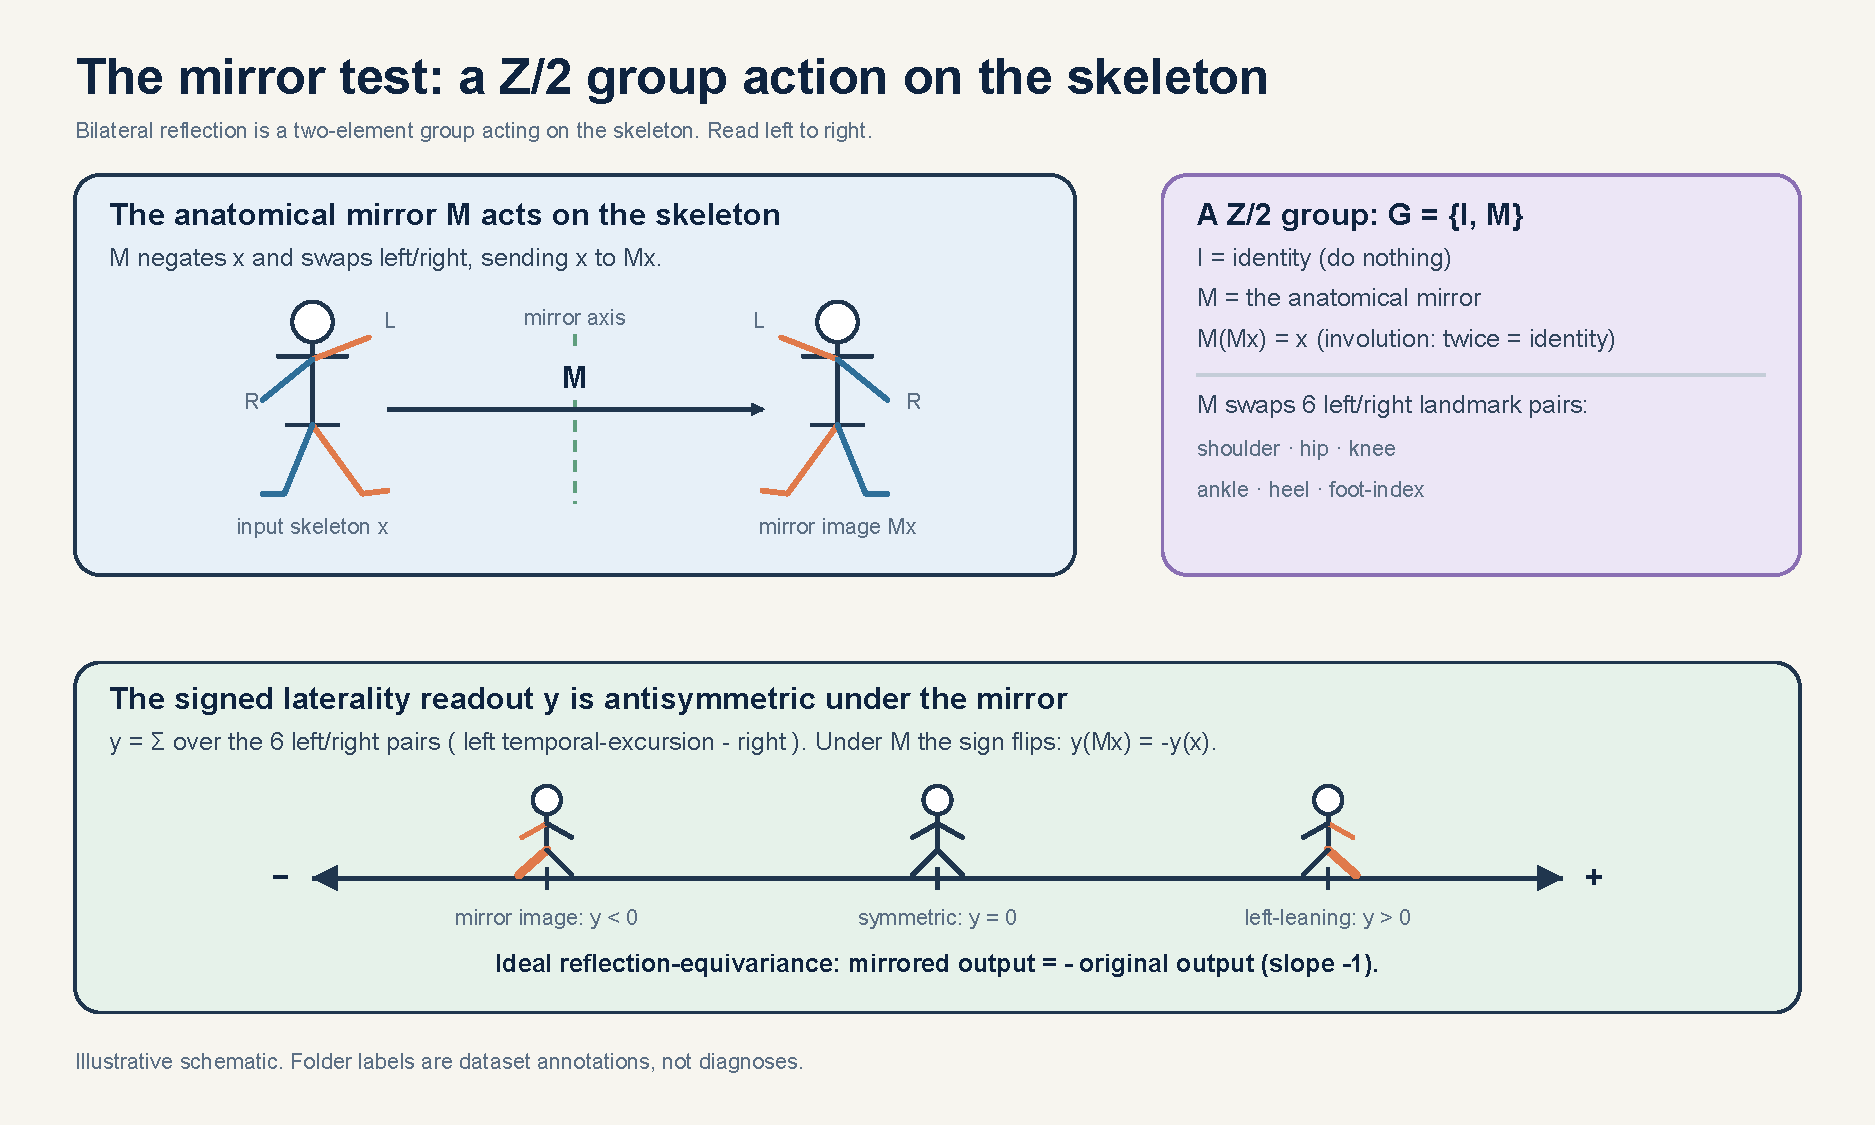
\includegraphics[width=0.60\linewidth]{fig1_group_action.pdf}
  \caption{Bilateral reflection as a $\mathbb{Z}/2$ group action: the signed laterality target is antisymmetric by construction, so ``encoding the symmetry'' means a decoded mirror slope of exactly $-1$.}
  \label{fig:group}
\end{figure}

\section{An audit protocol with ceiling, floor, and controls}

We probe a frozen S-JEPA (33-joint BlazePose, masked latent infilling, curriculum-trained; checkpoint fingerprint \texttt{7d13841a\ldots}) on five lanes: \textbf{A} learned per-pair token statistics; \textbf{B} raw-coordinate ceiling ($R^2\approx1$); \textbf{C} untrained-encoder floor; \textbf{D} side-blind pooled control; \textbf{E} landmark-missingness control. Estimation uses source-video-disjoint \texttt{GroupKFold} with an SVD-solver ridge and \textbf{repeated} shuffled CV over the \emph{fixed} cohort (10 reshuffles, mean $\pm$ a $t$-based across-reshuffle \emph{stability} interval, $\mathrm{df}=9$); the interval reflects partition sensitivity, not population sampling, and overlap is a stability heuristic, not a significance test \citep{bengio2004variance}. Pre-registered gates: A beats C by $\ge0.05$; A reaches $\ge80\%$ of B; sign correct on $\ge75\%$ of held-out sources. The primary cohort is the \textbf{626} sequences / \textbf{93} videos the encoder trained on (transductive); a 642 superset is a robustness view.

\section{E1: the symmetry does not emerge}

\begin{table}[h]
  \centering
  \caption{E1 laterality probe (626 primary).}
  \label{tab:e1}
  \begin{tabular}{lr}
    \toprule
    Lane & Repeated-CV $R^2$ (stability interval) \\
    \midrule
    A --- learned & \textbf{0.198 [0.175, 0.221]} \\
    C --- untrained floor & \textbf{0.245 [0.214, 0.275]} \\
    D --- pooled & 0.101 [0.089, 0.114] \\
    E --- missingness & 0.202 [0.173, 0.231] \\
    B --- raw ceiling (single-partition sanity check) & $\approx$1.000 \\
    \bottomrule
  \end{tabular}
\end{table}

Mirror slope $-0.70$ (no flip); sign consistency $0.58$. \textbf{All three gates fail}---under repeated CV the learned feature sits below the untrained floor in mean, with overlapping stability intervals (a partition-stability heuristic, not a significance test). The single-partition ordering $A>C$ \emph{reverses} under repetition; an alpha sweep (score rising monotonically from $-2.04$ to $+0.27$ only under heavy regularization) is consistent with a weak, collinear feature. The missingness control $E$ ($0.202$) has a mean close to $A$ ($0.198$), flagging possible visibility confounding and corroborating the null. A \textbf{robust informative null}.

\section{E2/E3: recover the geometry by construction}

\paragraph{Frame-averaged read-out (E2).} With $\Phi(x)=A(x)-A(Mx)$, a linear read-out on $\Phi$ has mirror slope \textbf{exactly $-1$ for any nonzero weights}. It reaches $R^2=0.273$ $[0.253,0.294]$, above the free read-out $0.198$ $[0.175,0.221]$ in repeated-CV mean (disjoint stability intervals---a partition-stability heuristic, not a formal test). The controls are consistent with the antisymmetric \emph{constraint} as the source of the gain (they do not establish a causal decomposition): the symmetric part $\Psi$ scores $0.015$ (slope $+1$, single-partition); an unconstrained $\ge$-capacity MLP that sees both mirror passes but is untied collapses to $0.047$ (slope $-0.43$, single-partition); the exactly-tied nonlinear head adds nothing over linear $\Phi$. The benefit over \emph{learning} is only suggestive, though: frame-averaging the \emph{untrained} encoder already reaches $0.219$ $[0.175,0.264]$ (overlapping interval). Point-estimate, $\Phi$ exceeds free $A$ by $0.075$; the architecture and learned-encoder contrasts ($\Phi_\text{floor}-A$, $\Phi-\Phi_\text{floor}$) are $0.021$ and $0.054$ with overlapping intervals---so the \emph{learning} benefit is suggestive, not decisive.

\paragraph{Frame-averaged encoder (E3.1).} Averaging the encoder, $E'(x)=\tfrac12(E(x)+\sigma\!\cdot\!E(Mx))$, is \textbf{exactly token-equivariant with zero retraining} (equivariance error $0.0$); the feature splits exactly into antisymmetric ($\ell-r$) and symmetric ($\ell+r$) blocks. The antisymmetric block \emph{corresponds to} E2's $\Phi$---it is one half of $\Phi$'s $\ell-r$ sub-block (up to standardization), while $\Phi$ additionally antisymmetrizes the $\ell+r$ block.

\paragraph{Augmentation does not induce it (E3.2, single-seed).} Retraining Stage-0 with reflection augmentation ($p{=}0.5$ vs $0.0$, one switch) changes the loss but not the geometry: the augmented and untrained axes have similar repeated-CV means ($0.062$ $[0.011,0.114]$ vs $0.078$ $[0.013,0.144]$; overlapping stability intervals), so the negative rests on the mirror slope, which moves no closer to $-1$ (the \emph{untrained} encoder is closest, $-0.82$; the augmented arm furthest, $-0.51$---in this single-seed arm, slope proximity is not evidence of learned equivariance, consistent with sensitivity to feature geometry). A single-seed negative.

\section{Synthesis and takeaway}

\begin{figure}[t]
  \centering
  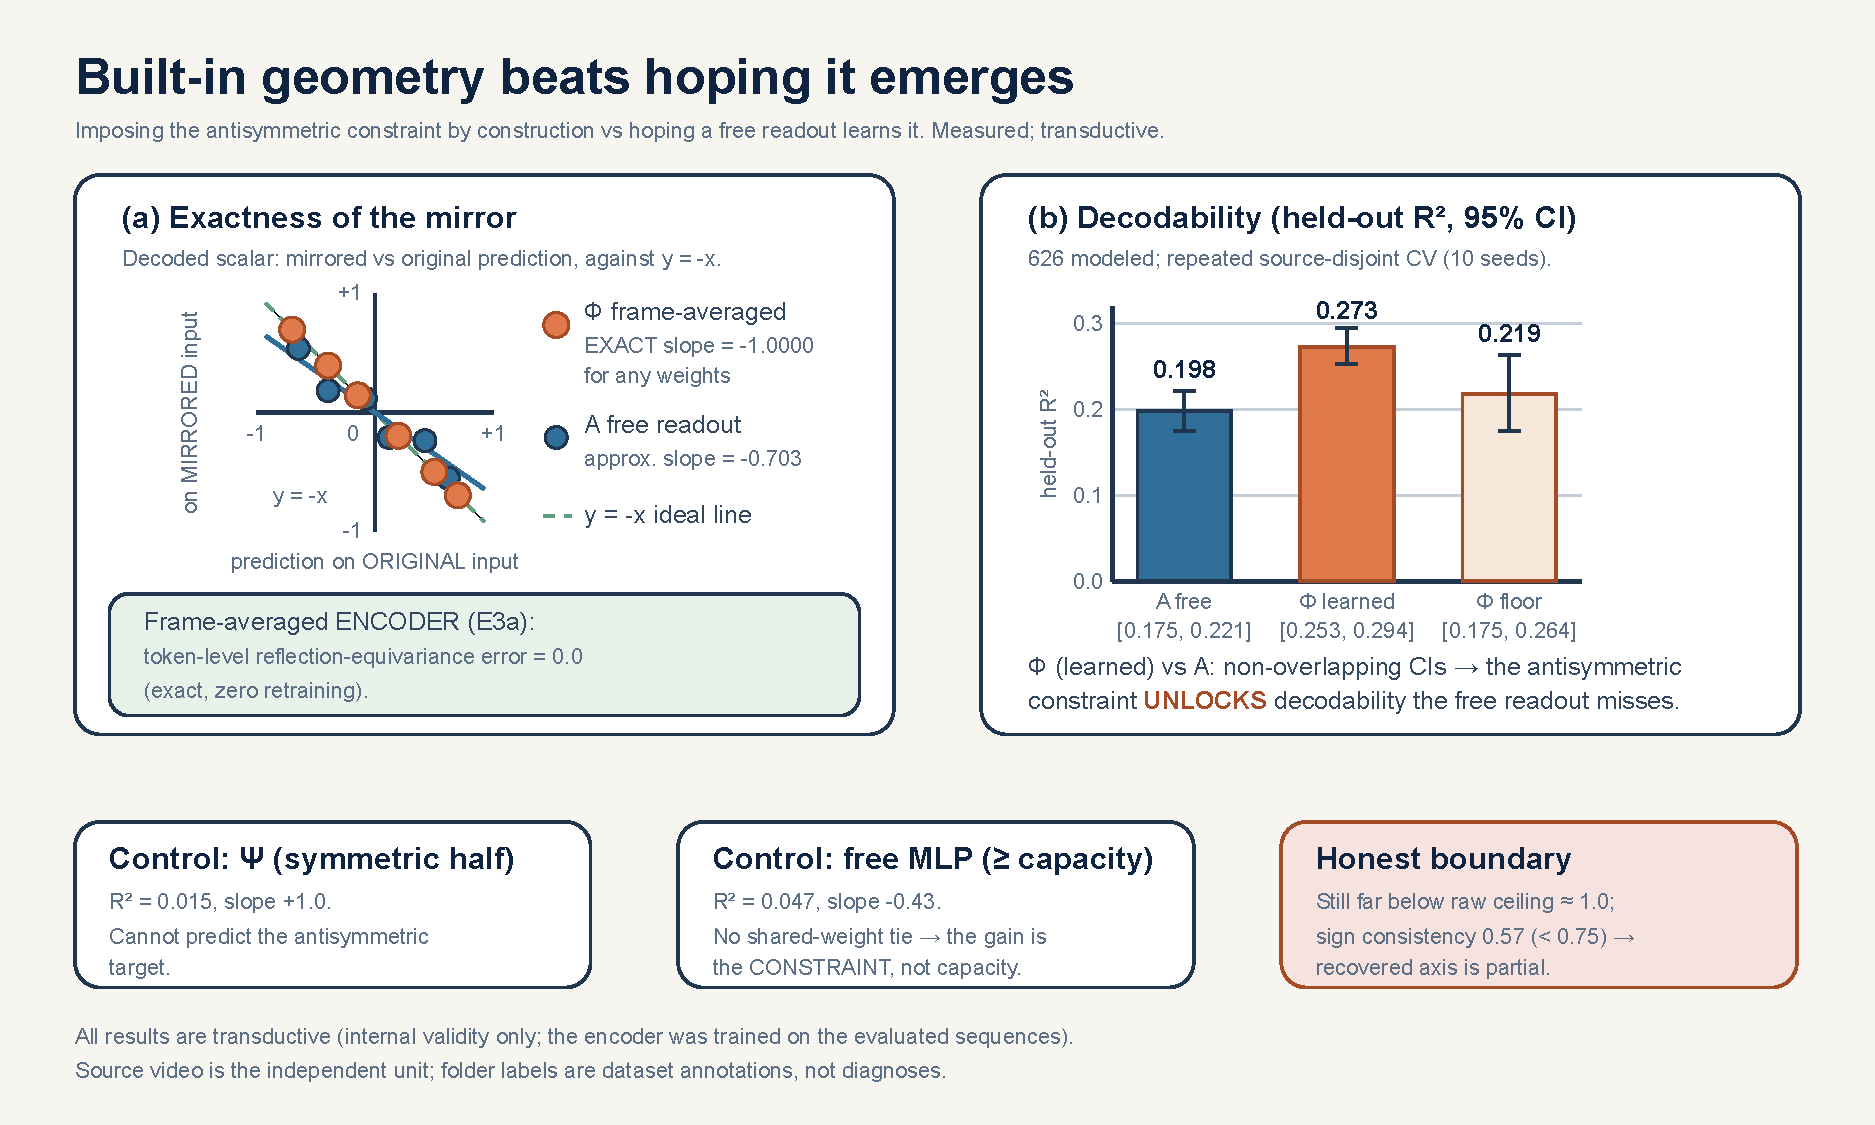
\includegraphics[width=0.72\linewidth]{fig5_builtin_beats_emergent.pdf}
  \caption{Built-in beats emergent, at both the read-out and the encoder. Emergent (E1/E3.2): at or below floor, slope not $-1$. Built-in (E2/E3.1): frame averaging recovers exact antisymmetry.}
  \label{fig:builtin}
\end{figure}

The four experiments form a $2\times2$ grid (Fig.~\ref{fig:builtin})---symmetry in the read-out or the encoder, hoped-for or built-in. \emph{Read-out}: emergent E1 has slope $-0.70$ with learned $\approx$ floor (intervals overlap), while built-in E2 has slope $-1.0000$ and $0.273>0.198$. \emph{Encoder}: emergent E3.2 has slope not toward $-1$ and axis $\le$ floor, while built-in E3.1 has token error $0.0$ (exact). In the audited system (single checkpoint; single-seed augmentation arm), standard and reflection-augmented self-supervision leave bilateral symmetry un-learned; frame averaging recovers it to machine precision at the read-out or encoder. The constructive claim is general; the negative is scoped to what we tested. For geometry-aware world models of articulated bodies, symmetry is cheap to \emph{impose} and---at least here---not reliably obtained by \emph{hoping} it emerges: \textbf{build the geometry in; don't hope it emerges.}

\section*{Ethics and limitations}

Results are transductive (internal validity only; no generalization claim). The dataset (GAVD \citep{ranjan2025gavd}) provides annotations and public YouTube URLs, not raw video; users retrieve media independently under YouTube's terms; we use derived pose sequences, infer no identity, and redistribute no raw or identity-bearing frames. \textbf{No institutional ethics determination or completed data-use review is yet on record; both must be resolved before submission.} Condition folder labels are dataset annotations, not diagnoses; the independent unit is the source video, not the individual; no clinical claim is made.

{\small
\bibliographystyle{plainnat}
\bibliography{../references}
}

\end{document}
